\BeginSection{Введение}
\begin{frame}[t]{Задача тематического моделирования}
\textbf{Дано:}
\begin{itemize}
    \item $D$ --- коллекция текстовых документов
    \item $W$ --- множество уникальных термов коллекции
    \item $n_{dw}$ --- число вхождений слова $w$ в <<мешок слов>> документа $d$
\end{itemize}

\medskip
\textbf{Найти:}
множество тем $T$ и два семейства распределений:
\smallskip
\begin{itemize}
    \item $p(w \cond t)$ --- распределения термов в темах (матрица $\Phi$)
    \item $p(t \cond d)$ --- распределения тем в документах (матрица $\Theta$)
\end{itemize}

\[
p(w \cond d) = \sum_{t \in T} p(w \cond t)p(t \cond d) = \sum_{t \in T} \phi_{wt}\theta_{td}
\]

\smallskip
\textbf{Критерий:} максимум (регуляризированного) правдоподобия
\[
     \sum_{d\in D} \sum_{w\in d} n_{dw} \ln
        \Bigl(
        \sum_{t\in T}
            \phi_{wt}\theta_{td}
        \Bigr) + \sum \tau_i R_i(\Phi, \Theta)
    \;\to\; \max_{\Phi,\Theta}. 
\]

Гиперпараметры: список регуляризаторов $R_i$, их коэффициенты $\tau_i$, число тем $|T|$.
% \footnotetext{
% Воронцов К. В. Аддитивная регуляризация тематических моделей коллекций текстовых документов // Доклады РАН. 2014.}
\end{frame}


\begin{frame}[t]{Нерешённые проблемы ARTM}

\begin{enumerate}
    \item{На практике трудно подбирать сочетание регуляризаторов и коэффициента регуляризации \begin{itemize}
        \item {нужен опыт, знание <<лучших практик>>}
    \end{itemize}}
    \item{ отсутствует каноническая модель ARTM с набором регуляризаторов <<по умолчанию>> \begin{itemize}
        \item {которая решает большинство прикладных задач}
    \end{itemize}}
    \item{ Используемый набора критериев не отражает многокритериальность задачи}
    \item{Отсутствует свободно доступная библиотека, которая упрощала бы построение тематических моделей \begin{itemize}
        \item {В ряде случаев BigARTM является <<слишком>> гибкой}
    \end{itemize}}
\end{enumerate}
\textbf{Цель:} разработка технологии построения интерпретируемых  тематических моделей, применимых для решения широкого класса задач тематического моделирования.

\end{frame}



\BeginSection{Методология построения ТМ в библиотеке TopicNet}

\begin{frame}{Возможности TopicNet}

\textcolor{blue}{\url{github.com/machine-intelligence-laboratory/TopicNet/}}
\bigskip
\begin{itemize}
    \item{Построение тематических моделей посредством \textcolor{red}{кубов} (гиперкубов, кубов гиперпараметров) и дерева эксперимента}
    \item{\textcolor{red}{Рецепты моделирования}: задание эксперимента при помощи текста}
    \item{\textcolor{red}{Многокритериальный отбор} тематических моделей}
    \item{Сохранение дерева эксперимента на диск}
    \item{Поддержка пользовательских регуляризаторов и критериев качества}
    \item{Средства визуализации}
\end{itemize}
\footnotetext{V. Bulatov, V. Alekseev, K. Vorontsov, D. Polyudova, E. Veselova, A. Goncharov, E. Egorov. \textbf{TopicNet: Making Additive Regularisation for Topic Modelling Accessible} // LREC 2020}
\end{frame}


\begin{frame}[t]{Cube: чертёж и инкубатор}

Куб задаёт многомерное пространство поиска (гиперкуб параметров) и осуществляет его обход (например, полным перебором всех точек). \\
\medskip
Координатами в пространстве поиска могут быть:

\begin{minipage}{0.5\textwidth}
{\small
    \begin{itemize}
        \setlength\itemsep{0em}
        \item число тем при инициализации модели
        \item неизвестный коэффициент определённого регуляризатора
        \item траектория регуляризации: \begin{itemize}
            \item номер итерации % (с какого момента обучения включается регуляризатор)
            \item скорость изменения коэффициента % регуляризации
        \end{itemize}
    \end{itemize}
}
\end{minipage}
\begin{minipage}{0.4\textwidth}
\begin{tikzpicture}
   \pic [text=blue!75!cyan] at (0,1) {annotated cuboid={
   width=300, height=200, depth=200, scale=.007, 
   xstring={$\{\tau_1,\tau_2,\tau_3\}$}, 
   ystring={$\{\xi_1,\xi_2\}$}, 
   zstring={$\{\eta_1,\eta_2\}$},, 
   }};
\end{tikzpicture}
\end{minipage}\\
\medskip
Куб, \textit{применённый} к тематической модели, порождает множество её потомков.

\begin{minipage}{0.1\textwidth}
    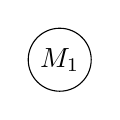
\begin{tikzpicture}
        \draw (0,0) circle [radius=0.4] node {$M_1$};
    \end{tikzpicture}
\end{minipage}
\begin{minipage}{0.05\textwidth}
    \scalebox{2}{+}
\end{minipage}
\begin{minipage}{0.4\textwidth}
    \begin{tikzpicture}
       \pic [text=blue!75!cyan] at (0,1) {annotated cuboid={
       width=300, height=200, depth=200, scale=.007,
          xstring=, ystring=, zstring=, 
       }};
       \draw[fill,blue] (-1,0)--(1.5,1) node[above]{$(\tau_1,\,\xi_2,\,\eta_1)$};
       \draw (-1,0) circle[radius=2pt];
    \end{tikzpicture}
\end{minipage}
\begin{minipage}{0.1\textwidth}
    \scalebox{2}{$\rightarrow$}
\end{minipage}
\begin{minipage}{0.1\textwidth}
    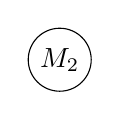
\begin{tikzpicture}
        \draw (0,0) circle [radius=0.4] node {$M_2$};
    \end{tikzpicture}
\end{minipage}

\end{frame}

\begin{frame}[t]{Многокритериальный отбор моделей в TopicNet}

В TopicNet введён специальный язык отбора моделей:

\begin{figure}[ht]
% \footnotesize
\raggedright
\texttt{TopicKernel@word.average\_contrast > 0.95 * MAXIMUM( \\
\hphantom{\ \ \ \ \ \ \ \ }TopicKernel@word.average\_contrast) \\
\hphantom{\ \ } and PerplexityScore@all < 1.1 * MINIMUM( \\
\hphantom{\ \ \ \ \ \ \ \ }PerplexityScore@all) \\
\hphantom{\ \ } and SparsityPhiScore@word -> max\\
\hphantom{\ \ } COLLECT 3} \\
\label{DSL-example}
\end{figure} 

Выражения соединены через \texttt{\colorbox{gray!30}{and}}. Выражения имеют вид:
{\small
    \begin{itemize}
        \setlength\itemsep{0em}
        \item Оптимизация: \texttt{\textcolor{blue}{Literal} -> MAX} (можно  \colorbox{gray!30}{\texttt{MAX}} или \colorbox{gray!30}{\texttt{MIN}})
        \item Ограничение: \texttt{\textcolor{blue}{Literal} > \textcolor{blue}{NumExpr} (можно \colorbox{gray!30}{>}, \colorbox{gray!30}{<} или \colorbox{gray!30}{=})}
            \begin{itemize}
            \item{\textcolor{blue}{NumExpr}} -- произвольное арифметическое выражение, использующее константы и/или литералы
            \item{Можно использовать специальные функции \texttt{MINIMUM, MAXIMUM, MEDIAN}}
            \end{itemize}
    \end{itemize}}
В конце можно указать требуемое количество моделей.
\end{frame}

\begin{frame}[t]{Многокритериальный отбор моделей в TopicNet}

Литералами могут быть:
{\small
    \begin{itemize}
        \setlength\itemsep{0em}
        \item Имя скора, присоединённого к модели:
            \begin{itemize}
            \item{Скоры из библиотеки BigARTM: чистота, контраст, разреженность, перплексия \dots}
            \item{Дополнительные критерии качества, реализованные в TopicNet}
            \item{Пользовательские критерии качества: \texttt{MyCustomScore}}
        \end{itemize}
        \item Структурные параметры модели: \texttt{model.num\_topics}
    \end{itemize}}
Дополнительные скоры, реализованные в TopicNet: 
{\small
    \begin{itemize}
        \setlength\itemsep{0em}
        \item Различность тем: среднее расстояние до ближайшей темы, среднее попарное расстояние между темами (метрики расстояния: Йенсен-Шэннон, Хэллингер, L2, косинусная близость)
        \item \textcolor{blue}{Анализ верхних токенов}: \texttt{JaccardSimilarityScore}, \texttt{BleiLaffertyScore}, \texttt{LogLift}, \textcolor{blue}{\texttt{TopTokensCoherenceScore}}
        \item \textcolor{red}{Внутритекстовая когерентность}: \texttt{IntratextCoherenceScore}.
        \item Качество кластеризации: \texttt{CalinskiHarabaszScore}, \texttt{SilhouetteScore}
        \item Расстояние до известных неинформативных распределений: равномерные $\phi_{wt}$, $\theta_{td}$, $p(t)$; эмпирическая частота токенов в коллекции
        \item Теоретико-информационные критерии: BIC, AIC, MDL, энтропия
    \end{itemize}}
\end{frame}

\begin{frame}[t]{Анализ верхних токенов}

Верхние токены (top-tokens) темы $t$: множество $Q_t$, состоящее из небольшого числа (как правило, 10) самых вероятных её токенов.\\

\[
\textup{LogLift}(t) = \sum_{w\in Q_t} \log \frac{\phi_{wt}}{P(w)}
\]
где $P(w)$ ---  средняя частота слова $w$ по коллекции.
\[
\textup{BleiLaffertyScore}(t) = \sum_{w\in Q_t} \phi_{wt} \log \bigg( \frac{\phi_{wt}}{\sqrt[T]{\prod_k \phi_{wk}}}\bigg)
\]

Две из возможных разновидностей когерентности:\\
\[
C_{UMass} = \sum_{w,v \in Q_t} \frac{\log P(w, v) + \epsilon}{P(w)}, \quad
C_{UCI} = \sum_{w,v \in Q_t} \frac{\log P(w, v) + \epsilon}{P(w)P(v)},
\]
где $\phi_{wt} > \phi_{vt}$, а $P(w, v)$ --- парная сочетаемость токенов $w$ и $v$ (основанная на счётчиках совместной встречаемости в скользящем окне).

\end{frame}

\begin{frame}[t]{Недостатки традиционной когерентности}

\begin{figure}
    %\begin{tabular}{p{7.5cm}p{3.5cm}}
        \includegraphics[width=0.5\textwidth]{doc11358_topic0.png} %&
        % 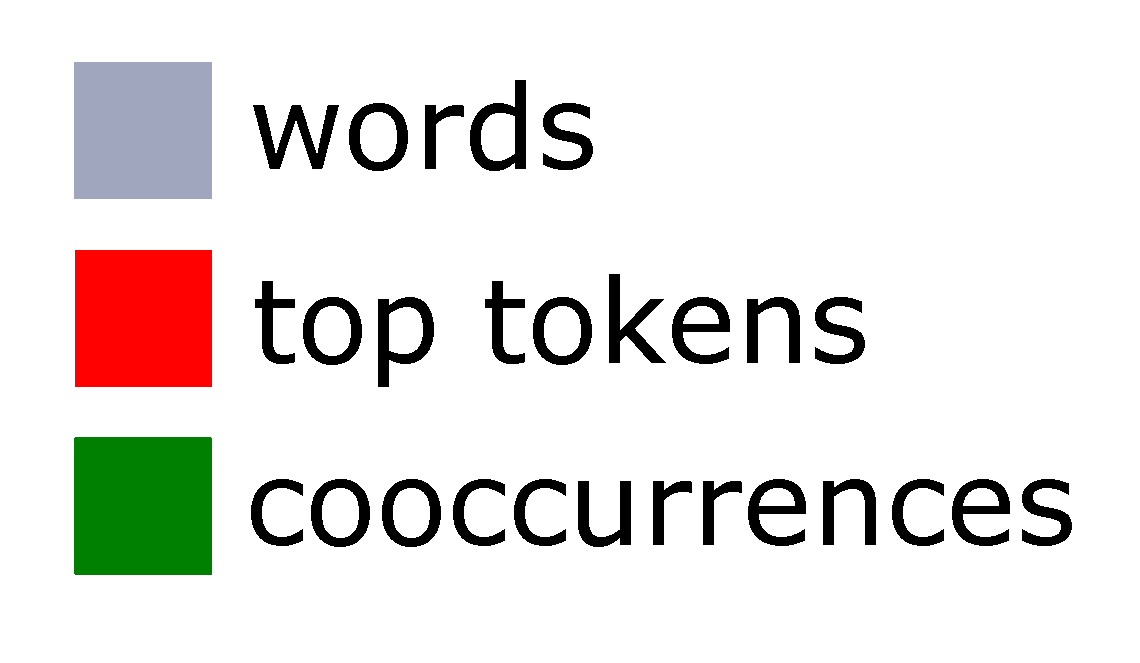
\includegraphics[width=0.25\textwidth]{legend.eps} \\
    %\end{tabular}
\end{figure}
\vspace{-7pt}
Словопозиции обозначены серо-синим цветом, словопозиции верхних слов показаны красным цветом, зелёным цветом показаны словопозиции, имеющие ненулевой вклад в расчёт когерентности.

Доля <<опорных>> слов --- порядка 1\% по всем темам, порядка 1/1000 для отдельной темы

\footnotetext{V. Alekseev, V. Bulatov, K. Vorontsov \textbf{Intra-text coherence as a measure of topic models’ interpretability} // Dialogue 2018}
\end{frame}
\begin{frame}[t]{Внутритекстовая когерентность}%

\small{
Усредним разброс $\mathrm{Var}(\phi_{w_i t}, \dots \phi_{w_{i+k} t})$ по всем окнам $[w_i, w_{i+1}, w_{i+2}, \dots, w_{i+k-1}, w_{i+k}]$ и всем документам. Получаем одну из возможных мер внутритекстовой когерентности $\textup{SemantiC}_{Var}(t)$, более чувствительную к изменениям тематической модели.
} \vspace{-7pt}
\begin{figure}
\begin{tabular}{cc}
\setlength\tabcolsep{0pt} % default value: 6pt
 \includegraphics[width=54mm]{images/segm_newman.png}  &   \includegraphics[width=54mm]{images/segm_var.png} 
\end{tabular}
    \caption{Сравнение различных мер когерентности и качества сегментации, нарисованное как функция от степени деградации тематической модели $\alpha$. }
\end{figure}
\footnotetext{V. Alekseev, V. Bulatov, K. Vorontsov \textbf{Intra-text coherence as a measure of topic models’ interpretability} // Dialogue 2018}
\end{frame}

\begin{frame}[t]{Дерево эксперимента в библиотеке TopicNet}

Процедуру применения куба и отбора моделей можно повторять. Тогда цепочка кубов образует многостадийный эксперимент.

\begin{tabular}{cc}
\setlength\tabcolsep{0pt} % default value: 6pt
\includegraphics[width=0.5\textwidth]{images/perplexity_tree.png} & 
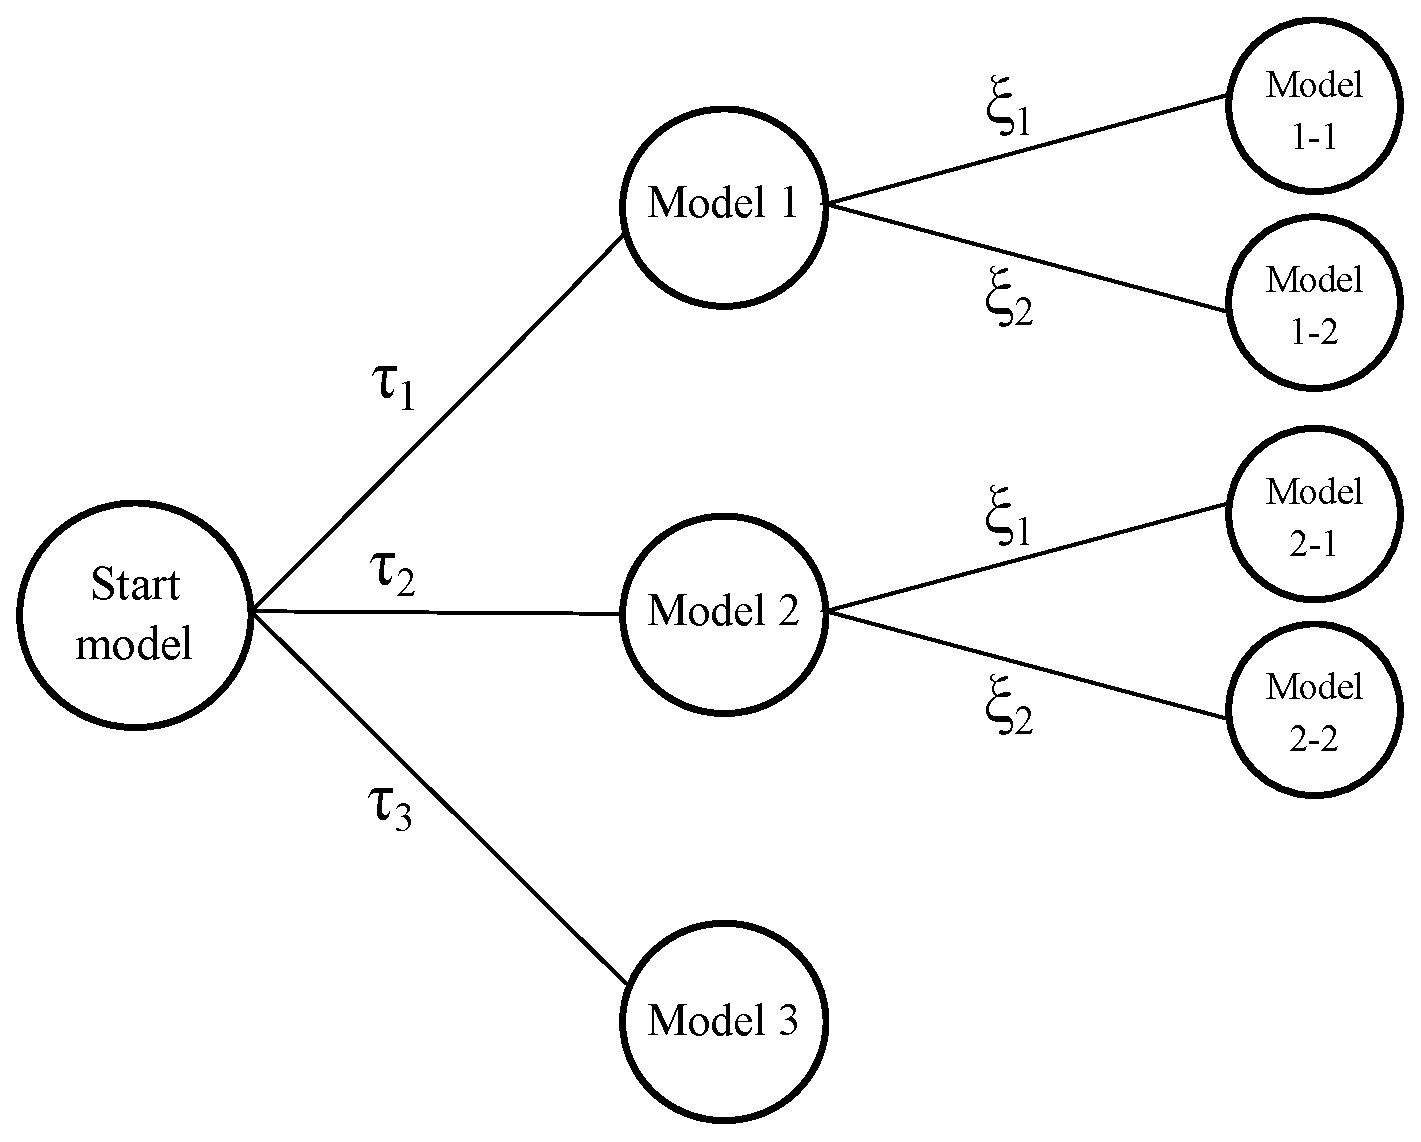
\includegraphics[width=0.45\textwidth]{training_scheme_example.eps}
\\
\footnotesize{Перплексия многостадийного эксперимента}
     & 
\footnotesize{Схема дерева эксперимента} \end{tabular}\\
\medskip
Рецепт --- это шаблон дерева эксперимента, переносимый на другие коллекции.
\end{frame}




\begin{frame}[t]{Относительные коэффициенты регуляризации}
\footnotesize

Документ может содержать не только слова, но и токены других модальностей (словосочетания, авторы, тэги, \dots).
Регуляризованное правдоподобие для мультимодального случая:

\[
L(\Phi^m, \Theta) = \sum_m \tau_m \sum_{d\in D} \sum_{w \in W^m} n_{dw} \log \sum_{t \in T} \phi_{wt}^{(m)} \theta_{td}
+
\sum_{i} \tau_i R_i(\Phi, \Theta)
\rightarrow \underset{\Phi, \Theta}{\mathrm{max}}
\]

где коэффициенты $\tau_m$ показывают \textit{вес} модальности $m$. Общие формулы M-шага:
\[
\theta_{td} = \norm_{t \in T} \Bigg(
    \sum_m n_{td}^{(m)} + \sum_{i=1}^k \tau_i \theta_{td} \frac{\partial R_i}{\partial \theta_{td}}
\Bigg), \quad \phi_{wt}^{(m)} = \norm_{w \in W^m}\Bigg(
    n_{wt}^{(m)} + \sum_{i=1}^k \tau_i 
    \phi_{wt}^{(m)} \frac{\partial R_i}{\partial \phi_{wt}^{(m)}}
\Bigg)
\]

\medskip
Идея: просуммировать каждое слагаемое по всем документам (для $\Theta$) или темам (для $\Phi$); отнормировать слагаемые на эту сумму. Тогда вместо $\tau_i$ будет  $\lambda_i$ - относительный коэффициент регуляризации, показывающий, \emph{во сколько раз} соответствующий регуляризатор влияет на оценку матриц больше, чем коллекция.

Случай $\phi_{wt}$ реализован в BigARTM, случай $\theta_{td}$~--- нет (поскольку $r_{id}$ недоступен при параллельной реализации).

\footnotetext{
Воронцов К. В. Аддитивная регуляризация тематических моделей коллекций текстовых документов // Доклады РАН. 2014.}
\normalsize
\end{frame}

\begin{frame}{Сглаживание, разреживание и веса модальностей}
Для некоторых важных случаев формула существенно упрощается!

\begin{table}[]
\begin{tabular}{l|c|c|}
         & \multicolumn{2}{c}{Управляющий параметр}                                                                                                      \\ \hline
         & $\tau$                                          & $\lambda$                                                                                   \\ \hline 
         &    &          \\[-5pt]
$\Phi$   & $\phi_{wt} = \norm_{w \in W}\Bigg(n_{wt} + \tau\Bigg)$    & $\phi_{wt} = \norm_{w \in W}\Bigg(n_{wt} + \lambda {\color{red}\frac{n}{|W||T|}}\Bigg)$    \\[15pt] \hline
         &    &          \\[-5pt]
$\Theta$ & $\theta_{td} = \norm_{t \in T} \Bigg(n_{td} + \tau\Bigg)$ & $\theta_{td} = \norm_{t \in T} \Bigg(n_{td} + \lambda {\color{red}\frac{n}{|D| |T|}}\Bigg)$ \\[15pt]  \hline
         &    &          \\[-5pt]
$\tau_m$ & $\theta_{td} = \norm_{t \in T} \Bigg(n_{td} + \tau n_{td}^{(m)}\Bigg)$ & $\theta_{td} = \norm_{t \in T} \Bigg(n_{td} + \lambda  {
    \color{red}\frac{n}{\sum_d n_d^{(m)}}
    } n_{td}^{(m)}\Bigg)$ \\[15pt]  \hline
\end{tabular}
\end{table}
Вывод: в этих случаях абсолютные коэффициенты и относительные эквивалентны. В частности, можно вычислить абсолютный коэффициент сглаживания $\Theta$, эквивалентный заданному относительному.
\end{frame}


\BeginSection{Таксономия обращений и относительные коэффициенты}


\begin{frame}{Таксономия обращений}
	\textbf{Дано:} две большие коллекции диалогов между клиентом и оператором (диалоги с госслужащими: 95k диалогов; техподдержка провайдера: 90k диалогов).\\
\texttt{\footnotesize
- где узнать статус поданного заявления\\
- Здравствуйте, меня зовут Юлия. Уточните ваш вопрос, пожалуйста.\\
- скажите пож, в каком разделе мне можно узнать статус поданного заявления
}\\
	\textbf{Найти:} иерархию интентов, входящих в коллекцию (двухуровневая иерархическая модель). \\
	
	\textbf{Критерии}: {\small\begin{itemize}
	    \item Интерпретируемая тематическая модель
	    \item Темы первого уровня описывают субъект диалога
	    \item  Темы второго уровня должны описывать действие, в котором заинтересован пользователь.
	    \item  \emph{Стратегия построения модели должна переноситься на похожие коллекции}
	\end{itemize}}
\footnotetext{A. Popov, V. Bulatov, D. Polyudova, E. Veselova. \textbf{Unsupervised dialogue intent detection via hierarchical topic model} // RANLP 2019}
\end{frame}

\begin{frame}{Дополнительные модальности}

Используется пять модальностей:
\begin{itemize}
    \item \texttt{@lemmatized} (просто слова)
    \item \texttt{@verb\_lemmatized} (слова-глаголы)
    \item \texttt{@noun\_lemmatized} (слова-существительные и слова-прилагательные)
    \item \texttt{@theme\_ngramms} ($n$-грамы с существительными и без глаголов)
    \item \texttt{@verb\_ngramms} ($n$-грамы с глаголами)
\end{itemize}

%{\footnotesize
%(информативные $n$-грамы выделены с помощью модифицированного алгоритма TopMine)}
\begin{table}[!t]
\begin{tabular}{|l|l|l|}\hline
                & Вес на первом уровне & Вес на втором уровне \\ \hline
\texttt{@lemmatized}     & 0.5                  & 0.5                  \\ \hline
 \texttt{@theme\_ngramms}   & 0.5                  & 0.5                  \\ 
\texttt{@noun\_lemmatized} & \textbf{0.5}                  & \textbf{0.1}                 \\ \hline
\texttt{@verb\_ngramms}    & \textbf{0.1}                  & \textbf{1}                    \\ 
\texttt{@verb\_lemmatized} & \textbf{0.1}                  & \textbf{1}                    \\ \hline
\end{tabular}
\caption{Относительные веса модальностей для двух уровней}
\end{table}

\end{frame}


\begin{frame}{Решение. Полученные темы для двух коллекций}

\begin{table}[!h]
\begin{tabularx}{\textwidth}{|X|X|}
  \hline
  \textbf{Тарифный план} & \textbf{Запись на приём к врачу} \\
  \hline
  \textsl{Как \textbf{сменить} тарифный план?} &   \textsl{Как \textbf{отменить запись}?}\\
  \textsl{Когда \textbf{произошло изменение} тарифного плана?} &   \textsl{Почему я \textbf{не могу записаться} на приём?}\\
  \textsl{Как часто можно \textbf{менять тарифный план}?} &  \textsl{\textbf{Не могу найти} в списке поликлинику №X?} \\
  \textsl{Когда \textbf{вступят в силу изменения} тарифного плана?} &    \textsl{Почему в списке \textbf{отсутствует специалист} X?} \\
  \textsl{Почему у меня \textbf{не получается изменить} тарифный план?} & 
  \textsl{Как \textbf{записать} на приём ребёнка?}\\
  \hline
\end{tabularx}
\caption{Различные подтемы темы верхнего уровня}
\label{topic_subtopic}
\end{table}
\normalsize

\end{frame}


\BeginSection{Качество тематических моделей с параметрами <<по умолчанию>>}

\begin{frame}{Конкуренты и <<параметры по умолчанию>>}

\begin{table}[h]
\begin{tabular}{|l|l|l|}
\hline
           & \multicolumn{1}{c|}{\begin{tabular}[c]{@{}c@{}}Jaccard measure\\ of topic dissimilarity\end{tabular}} & \multicolumn{1}{c|}{\begin{tabular}[c]{@{}c@{}}Average topic\\ coherence\end{tabular}} \\ \hline
TopicNet   & \textbf{0.00169}                                                                                               & -2.551                                                                                 \\ \hline
Gensim LDA & 0.01374                                                                                               & -2.747                                                                                 \\ \hline
STTM DMM   & 0.37541                                                                                               & -2.726                                                                                 \\ \hline
STTM PTM   & 0.02485                                                                                               & \textbf{-2.510}                                                                                 \\ \hline
STTM WNTM  & 0.01997                                                                                               & -3.572                                                                                 \\ \hline 
\end{tabular}
\caption{Сравнение качества различных моделей, построенных при помощи различных программных средств}
\end{table} 



\end{frame}


\begin{frame}{Изменение оптимизационной задачи ARTM}

Оказывается, когерентность можно повысить введением зависимости $\Theta = f(\Phi)$, где $f$ --- одна итерация M-шага, восстанавливающая $\Theta$ с фиксированной $\Phi$.

\begin{itemize}
\item Оценка интерпретируемости: обычно используется только матрица $\Phi$.
\item $\Theta$ может скомпенсировать <<плохую>> $\Phi$, а её качество при этом не контролируется
\end{itemize}
\medskip
Исходная оптимизационная задача:
\[
L(\Phi, \Theta ) + R(\Phi, \Theta ) \to \max_{\Phi, \Theta}.
\]
Новая оптимизационная задача:
\[
\begin{cases}
& L(\Phi, \Theta ) + R(\Phi, \Theta ) \to \max_{\Phi, \Theta},\\
& \Theta = f(\Phi),
\end{cases}
\]

\end{frame}

\begin{frame}[t]{EM-алгоритм при $\Theta=f(\Phi)$}

\begin{Theorem}
    Пусть функция $R(\Phi,\Theta)$ непрерывно дифференцируема, а $\Theta$ находится в функциональной зависимости от $\Phi$ согласно формуле    $\theta_{td}(\Phi)
    = \norm_{t\in T} \biggl( \sum_{w\in W} n_{dw} p_{tdw} \biggr)$.
    Тогда точка $\Phi$ локального максимума 
    удовлетворяет системе уравнений со вспомогательными переменными $h_w,\ \theta_{td},\ p_{tdw},\ c_{td},\ \gamma_{dw}$:
\[
    \phi_{wt} = \norm_{w\in W}
        \Biggl(\,
        \sum_{d\in D} n_{dw} p_{tdw} 
        + \underbrace{\sum_{d\in D} n_{dw} n_d^{-1} \phi_{wt}h_w (c_{td}-h_w\gamma_{dw})}_{
            \let\scriptstyle\textstyle
            \substack{\textup{псевдорегуляризатор}}
        } + 
            \phi_{wt} \frac{\partial{R}}{\partial{\phi_{wt}}}
        \Biggr)
\]
\end{Theorem}
Можно реализовать в BigARTM/TopicNet, введя фиктивный псевдорегуляризатор и положив \texttt{num\_document\_passes~=~1}.


\footnotetext{Ирхин И.А., Булатов В.Г., Воронцов К.В. \textbf{Аддитивная регуляризация тематических моделей с быстрой векторизацией текста} // Компьютерные исследования и моделирование, 2020}
\end{frame}



\begin{frame}{Влияние на тематическую модель}

\begin{figure}
\setlength\tabcolsep{0pt} % default value: 6pt
\begin{tabular}{cc}
Расстояние JS между темами & Разреженность $\Phi$\\
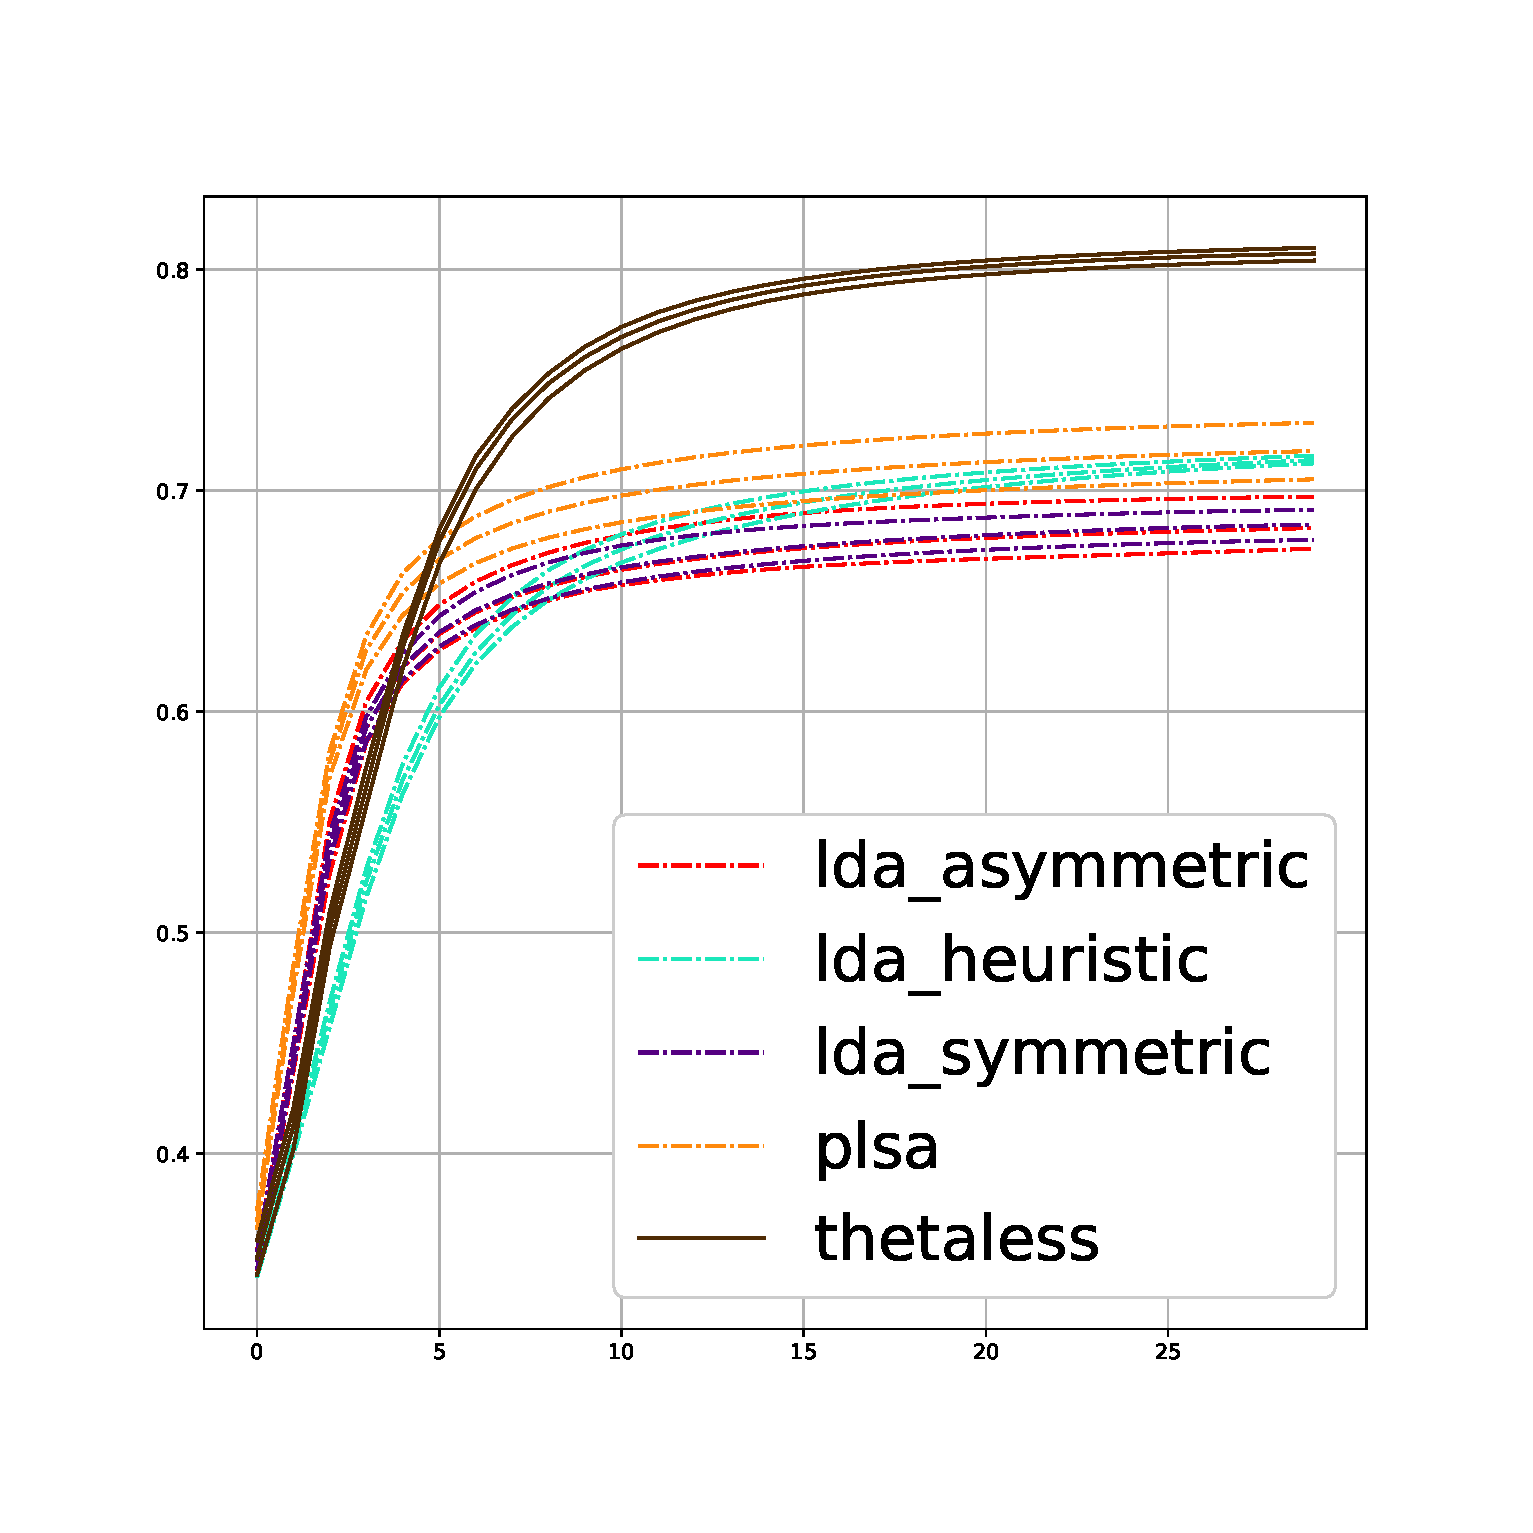
\includegraphics[width=54mm]{images/CH4_baselines_diversity_jensenshannon_False.eps} &
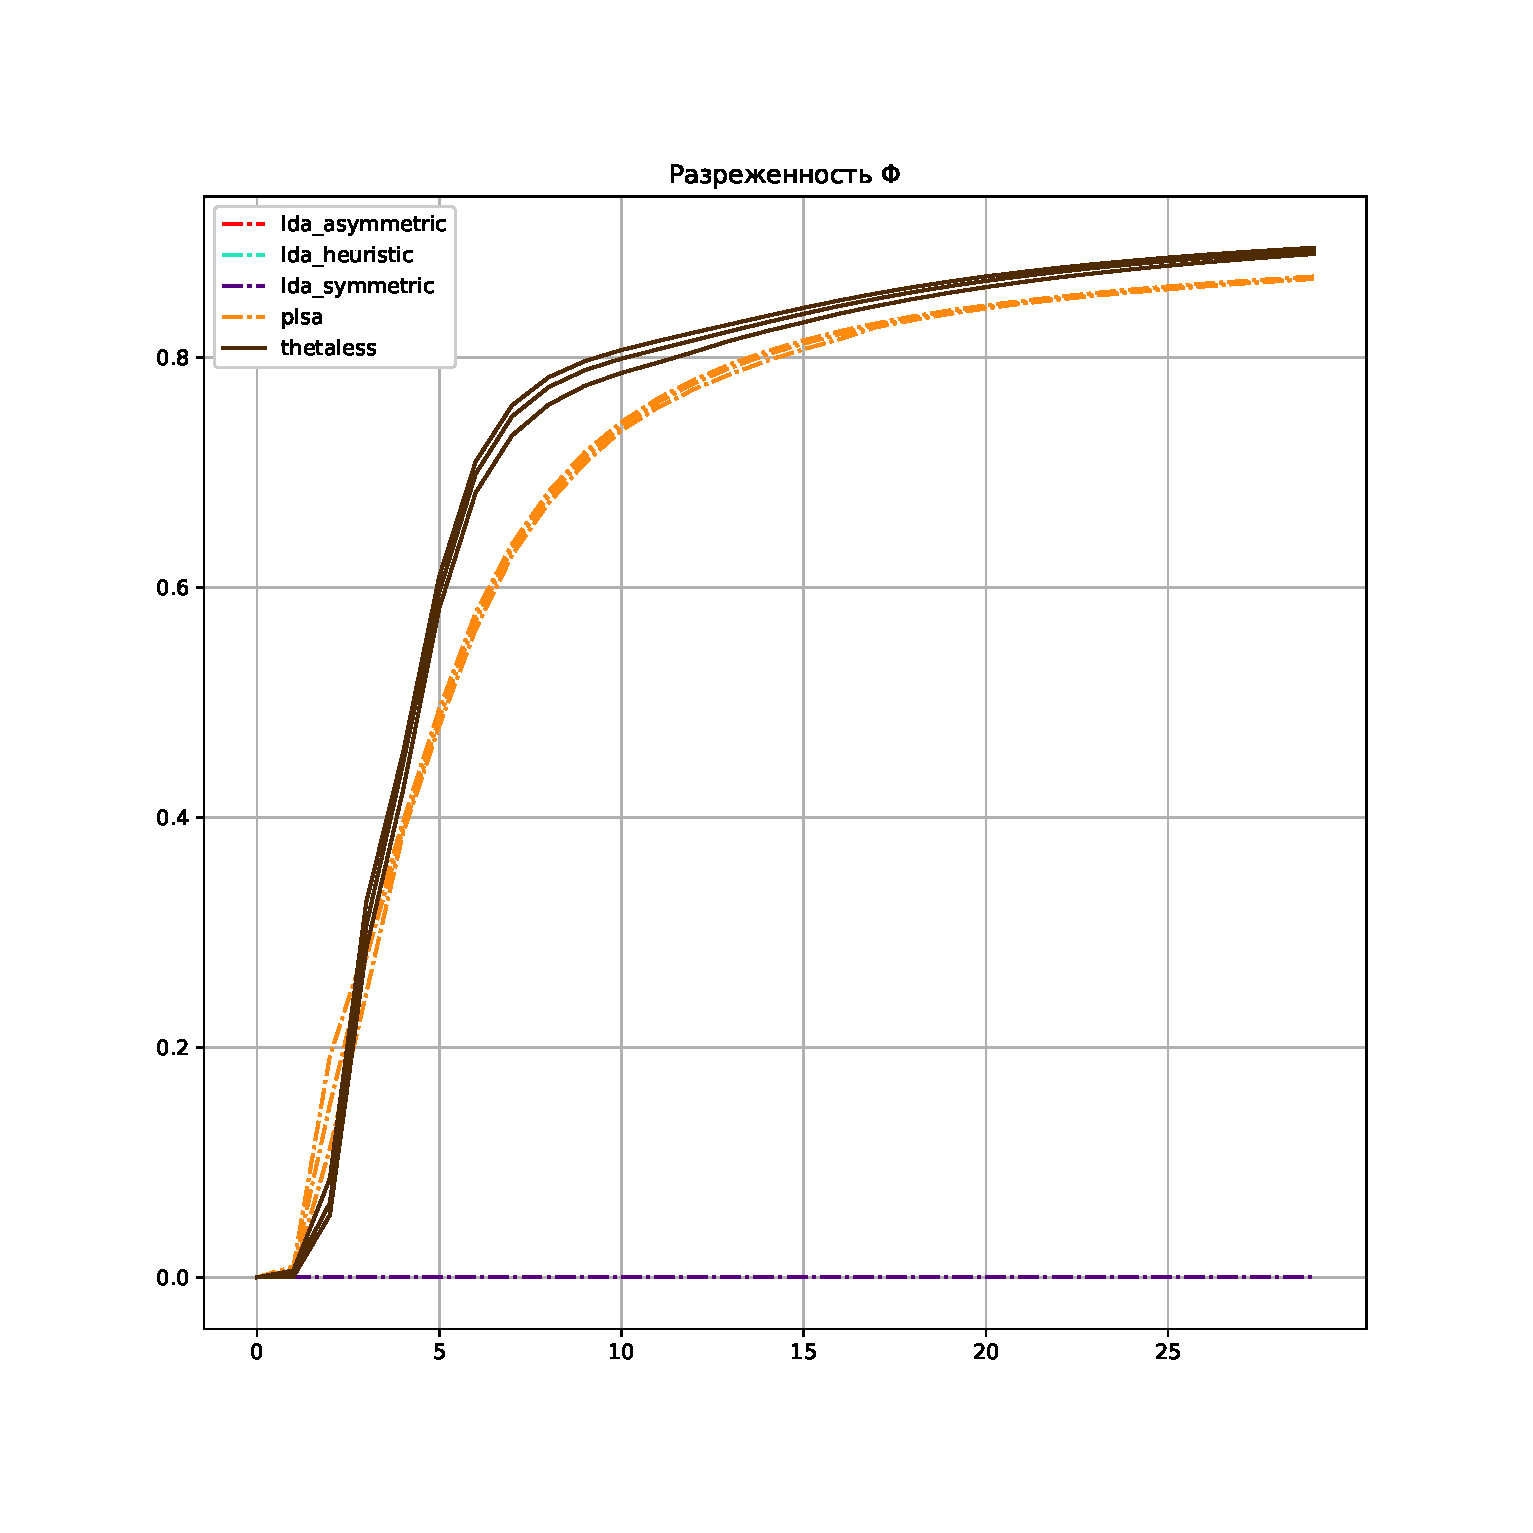
\includegraphics[width=54mm]{images/CH4_baselines_SparsityPhiScore.eps} \end{tabular}
\end{figure}
Сравнение с базовыми моделями (PLSA и LDA с 3 видами приоров). Каждой модели соответствуют три линии: среднее значение, минимум и максимум (по пяти случайным перезапускам)
\end{frame}

\begin{frame}{Влияние на тематическую модель}

\begin{figure}
\setlength\tabcolsep{0pt} % default value: 6pt
\begin{tabular}{cc}
Расстояние JS между темами & Разреженность $\Phi$\\
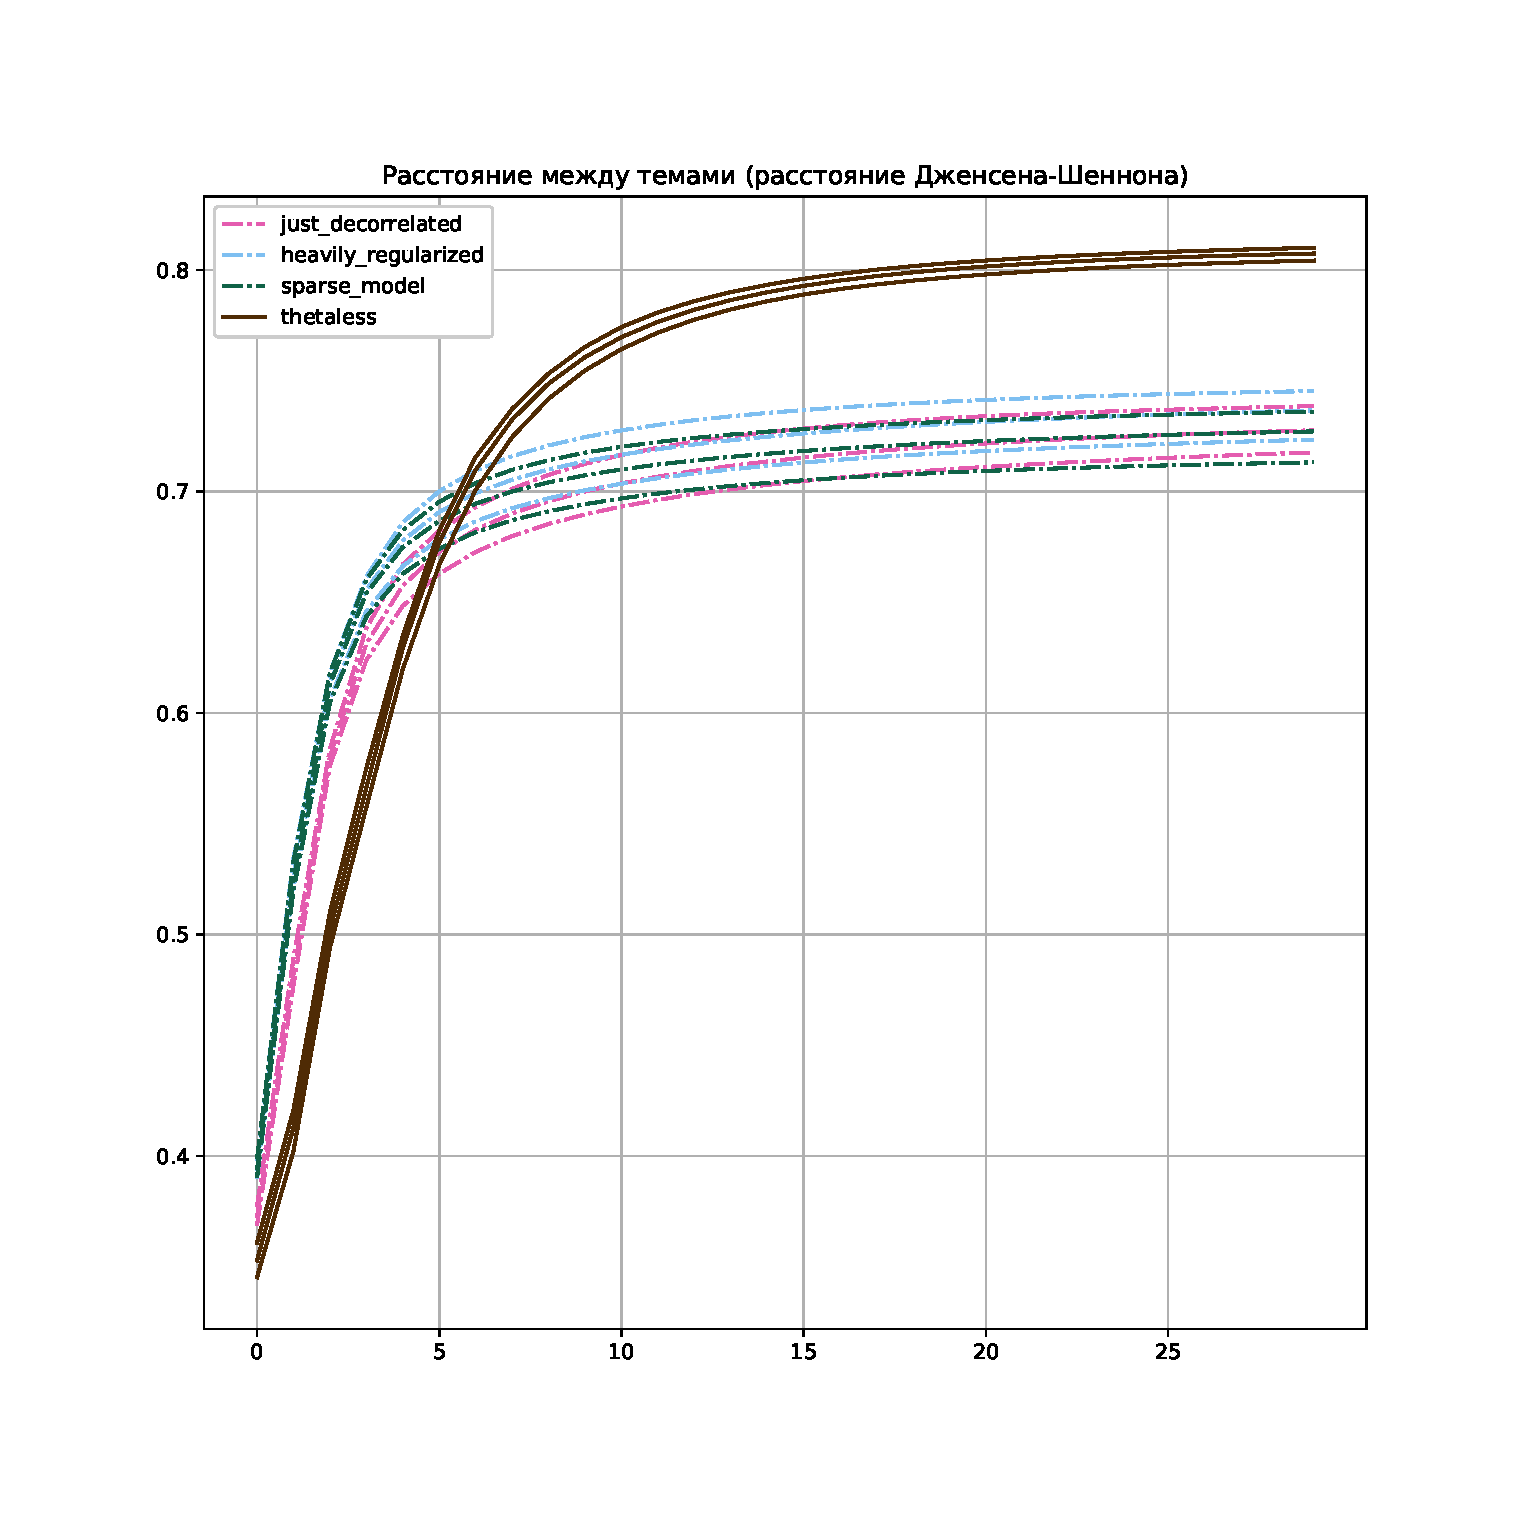
\includegraphics[width=54mm]{images/CH4_vs_regularized_diversity_jensenshannon_False.eps} &
\includegraphics[width=54mm]{images/CH4_vs_regularized_SparsityPhiScore.eps} \end{tabular}
\end{figure}
Сравнение с тремя аддитивно регуляризованными моделями
\end{frame}

\begin{frame}{Комбинирование с другими регуляризаторами}

\begin{figure}[t]
\setlength\tabcolsep{0pt} % default value: 6pt
\begin{tabular}{cc}
Расстояние JS между темами & Разреженность $\Phi$\\
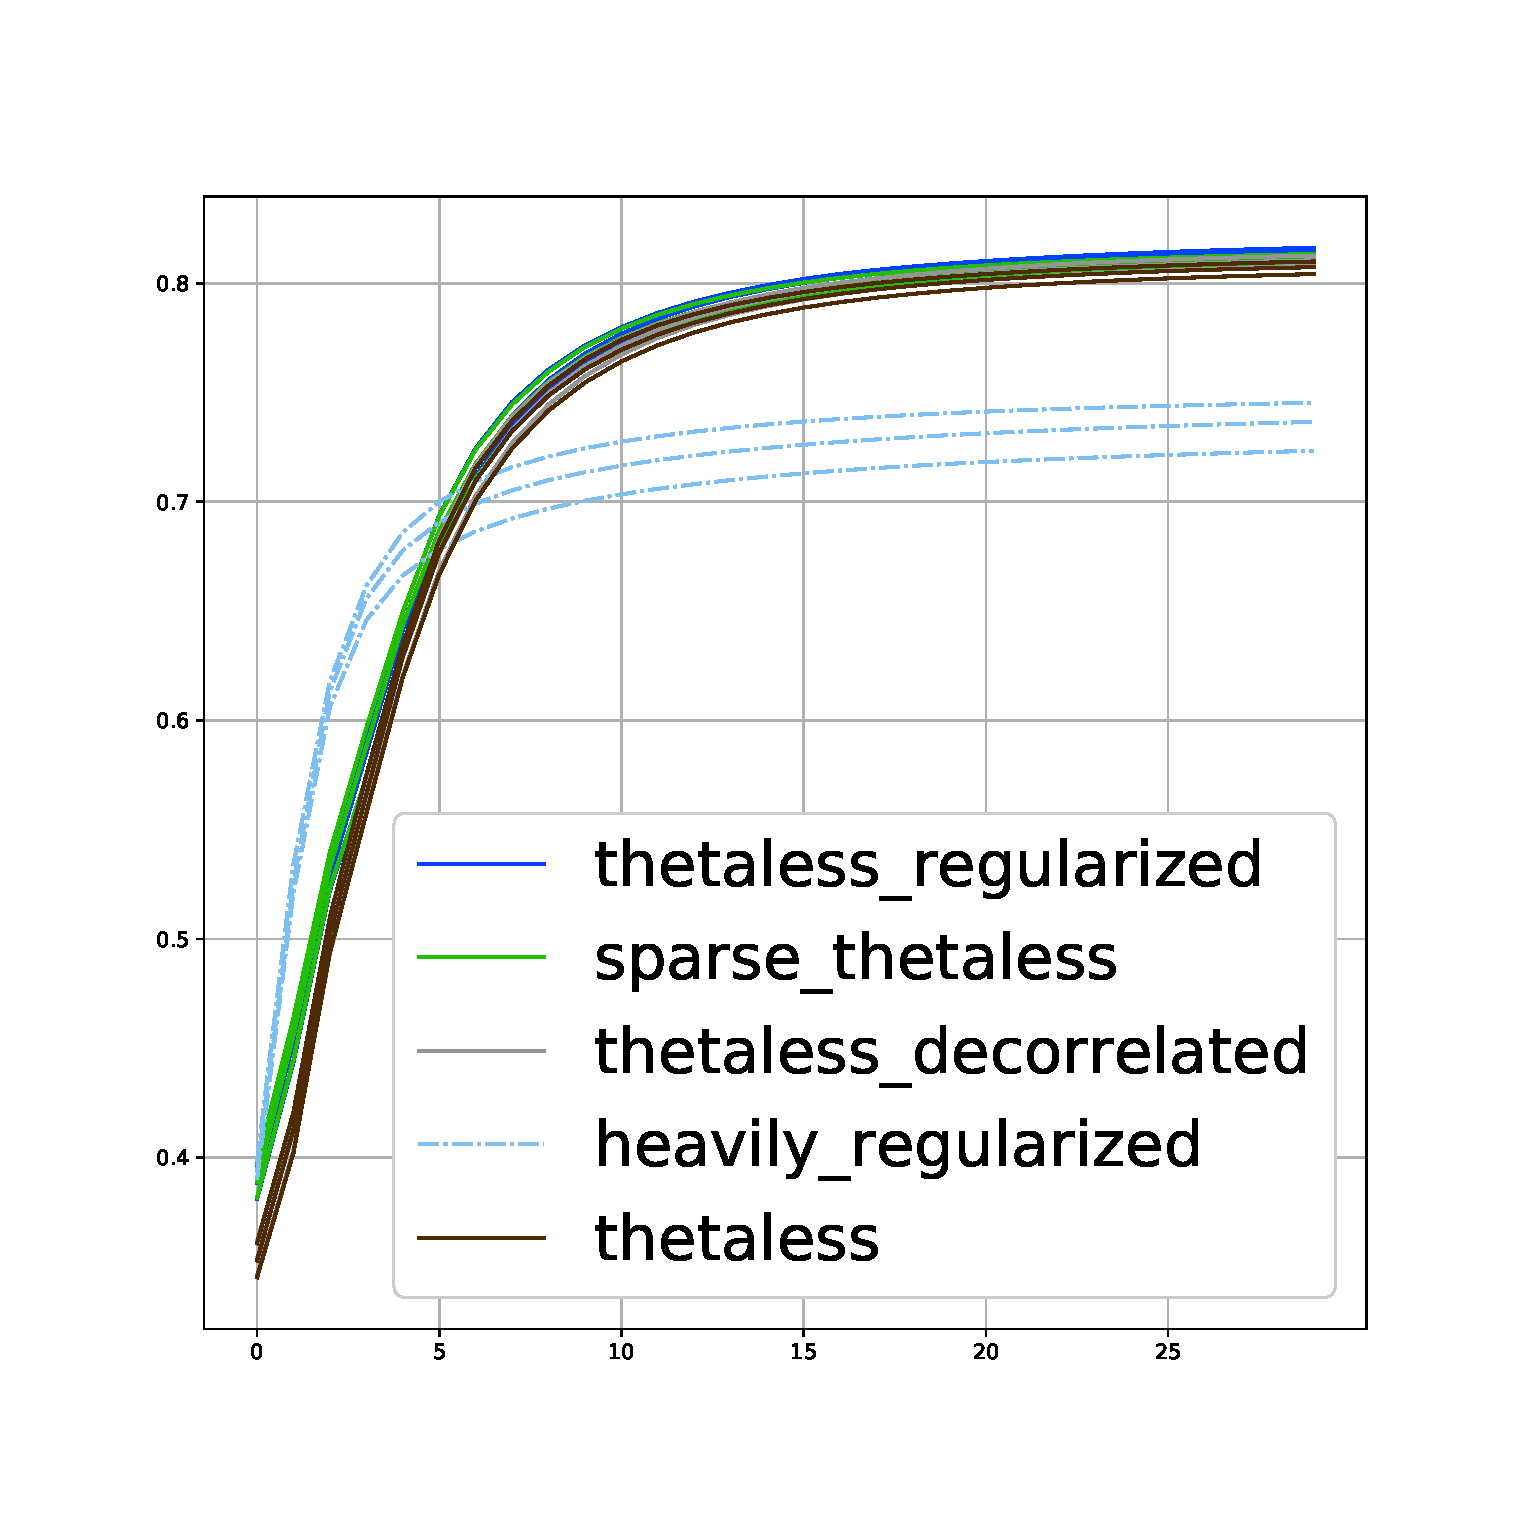
\includegraphics[width=54mm]{images/CH4_improved_diversity_jensenshannon_False.eps} &
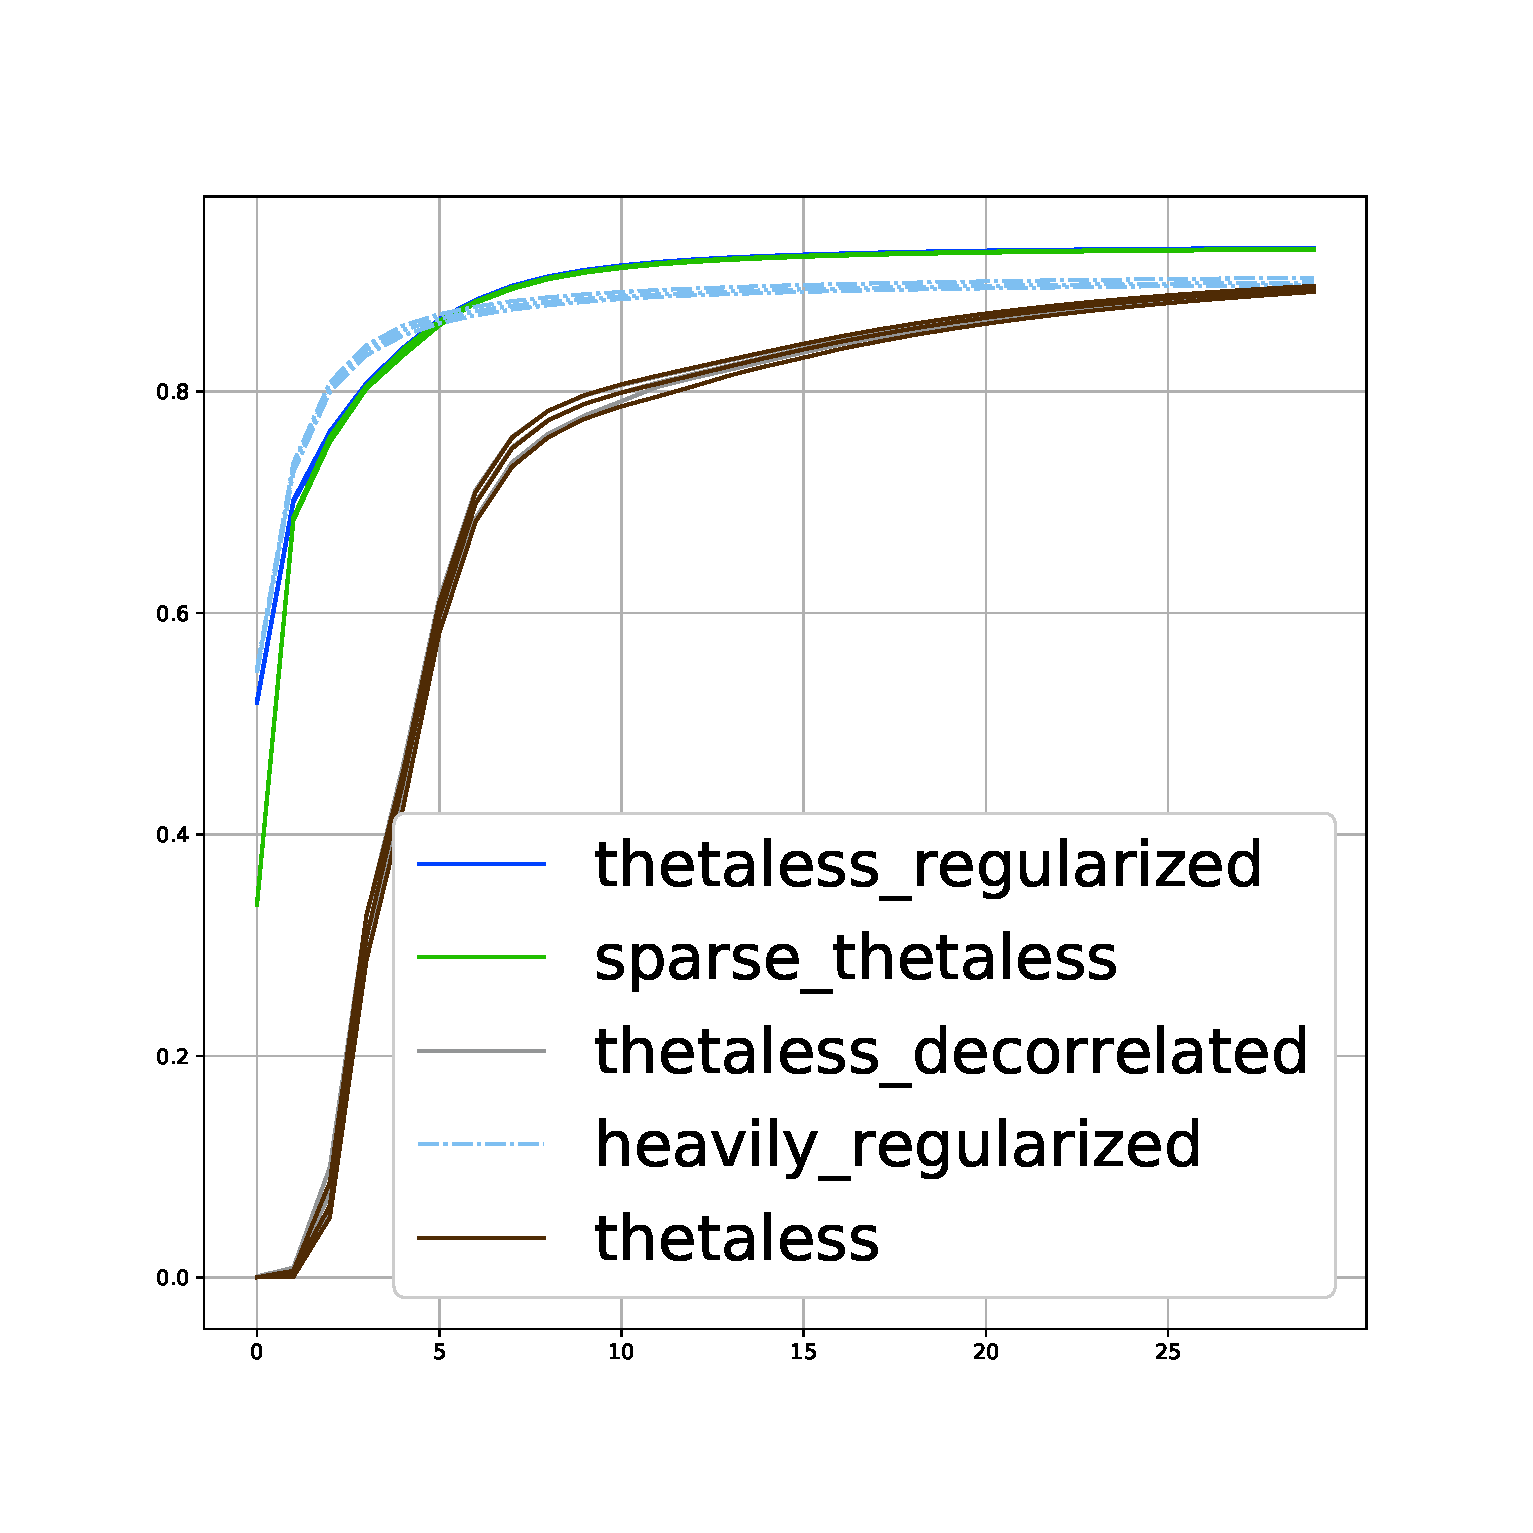
\includegraphics[width=54mm]{images/CH4_improved_SparsityPhiScore.eps} \end{tabular}
\end{figure}
% Псевдорегуляризатор успешно комбинируется с другими регуляризаторами ARTM, за счёт чего можно улучшить критерии качества ещё больше.

Тематическая модель с псевдорегуляризатором и традиционным набором регуляризаторов (сглаживание фоновых тем, разреживание предметных тем, декорреляция) выигрывает у аналогичного ARTM по разреженности.

\end{frame}

% \BeginSection{TopicNet и <<настройки по умолчанию>>}

\begin{frame}{Базовый рецепт с быстрой векторизацией}

\begin{table}[h]
\begin{tabular}{|l|l|l|}
\hline
                         & UMass & LogLift             \\ \hline
BaselineRecipe           & -3.145         & 29.217         \\ \hline
ThetalessBleiLafferty   & -2.075         & 31.143           \\ \hline
ThetalessLift           & \textbf{-1.805}  & \textbf{33.904} \\ \hline
LDA\_asymmetric\_symmetric & -2.446          & 21.388           \\ \hline
LDA\_asymmetric\_auto      & -3.078          & 24.321          \\ \hline
LDA\_symmetric\_symmetric  & -2.884          & 23.554         \\ \hline
LDA\_symmetric\_auto       & -2.279         & 21.738          \\ \hline
LDA\_auto\_symmetric       & -2.382           & 24.154          \\ \hline
LDA\_auto\_auto            & -2.749          & 25.458 \\ \hline
\end{tabular}
\caption{Сравнение моделей по ряду критериев качества. Повышение как UMass-когерентности так и LogLift означает улучшение модели. Также модели TopicNet превосходят GenSim по разреженности и различности тем.}
\label{tbl:better_baseline}
\end{table} 

\end{frame}



\begin{frame}
    \frametitle{Положения, выносимые на защиту}
\small
    \begin{itemize}
\item
    Методология построения тематических моделей, обеспечивающая формирование <<рецептов моделирования>> с автоматизированным подбором гиперпараметров по множеству критериев и отличающаяся использованием относительных коэффициентов регуляризации и кубов гиперпараметров.
\item
    Архитектура библиотеки TopicNet, обеспечивающая программную реализацию данной методологии и отличающаяся использованием удобного языка описания кубов гиперпараметров и возможностью создания пользовательских регуляризаторов и метрик качества на языке Python.
\item
    Универсальный рецепт моделирования, обеспечивающий многокритериальный выбор тематических моделей для широкого класса задач, отличающийся предварительной настройкой куба гиперпараметров по набору разнородных задач тематического моделирования.
\item
    Программная реализация нового критерия когерентности, обеспечивающая его эффективное вычисление и отличающаяся более полным использованием данных о сочетаемости слов внутри текстовых документов.
%\item
%    Программная реализация псевдорегуляризатора в библиотеке TopicNet, обеспечивающего быстрое однопроходное вычисление тематических векторных представлений документов и улучшение качества тематической модели по множеству критериев.
    \end{itemize}

    
\end{frame}


\begin{frame}[t]{Публикации и РИДы}
\footnotesize

Публикации в изданиях, индексируемых Scopus:
\begin{itemize}
    \smallskip\item  V. Alekseev, V. Bulatov, K. Vorontsov. Intra-text coherence as a measure of topic models’ interpretability  // Dialogue 2018

    \smallskip\item A. Popov, V. Bulatov, D. Polyudova, E. Veselova. Unsupervised dialogue intent detection via hierarchical topic model // RANLP 2019

    \smallskip\item V. Bulatov, V. Alekseev, K. Vorontsov, D. Polyudova, E. Veselova, A. Goncharov, E. Egorov. TopicNet: Making Additive Regularisation for Topic Modelling Accessible // LREC 2020

    \smallskip\item\color{red} И. А. Ирхин, В. Г. Булатов, К. В. Воронцов. Аддитивная регуляризация тематических моделей с быстрой векторизацией текста // Компьютерные исследования и моделирование, 2020
\end{itemize}

Зарегистрированные программы для ЭВМ в РФ:
\begin{itemize}
    \smallskip\item  Topic Net Cooking Machine  / Гончаров А. В., Булатов В. Г., Воронцов. К. В.; МФТИ. --- опубл. 17.09.2019, 2019662102

    \smallskip\item Система создания таксономии текстовой коллекции диалогового контактного центра / Гончаров А. В., Егоров. Е. О., Веселова. Е. Р., Булатов. В. Г.; МФТИ. --- опубл. 17.03.2020, 2020613851

    \smallskip\item Topic Net Viewers  / Гончаров А. В., Булатов В. Г., Воронцов. К. В.; МФТИ. --- опубл. 10.09.2019, 2019661840

\end{itemize}

\normalsize
\end{frame}
